\documentclass[
  %ignorenonframetext,
  aspectratio=1610,
]{beamer}

\usepackage{Helmholtz-AI}
%% extrapackages added from markdown frontmatter
\usepackage{fontawesome5}
\usepackage{xspace} 
\usepackage{lmodern}
\usepackage{graphicx}
\usepackage{booktabs}
\usepackage{tabularx}
\usepackage{array}
\usepackage{xspace}
\usepackage{verbatim}
\usepackage{listings}
\usepackage{pifont}
\usepackage{ulem}
\usepackage{media9}
\usepackage{enumitem}
% References
% \usepackage[
%   backend=biber,
%   url=true,
%   sorting=none,
%   ]{biblatex}
%   \addbibresource{references.bib}
\usepackage{hyperref}

\definecolor{applegreen}{rgb}{0.55, 0.71, 0.0}
\definecolor{cadmiumred}{rgb}{0.89, 0.0, 0.13}
  
\providecommand{\tightlist}{%
  \setlength{\itemsep}{0pt}\setlength{\parskip}{0pt}}

% add labels to itemize
\setlist[itemize,1]{label=\textbullet}
\setlist[itemize,2]{label=\textopenbullet}

\hypersetup{
  colorlinks=true,
  linkcolor=hgfblue,
  filecolor=Maroon,
  citecolor=hgfinformation,
  urlcolor=hgfmatter,
  pdfcreator={Till Korten}
  }

\usepackage{tikz}
\usetikzlibrary{positioning}
\usetikzlibrary{arrows.meta}

% LISTINGS SETUP (for code)
\lstdefinestyle{code}{
basicstyle=\ttfamily\footnotesize,
keywordstyle=\bfseries,
commentstyle=\itshape,
showstringspaces=false,
columns=fullflexible,
frame=single,
breaklines=true,
tabsize=2
}

% SHORTCUTS
\newcommand{\cmark}{\ding{51}} % checkmark
\newcommand{\xmark}{\ding{55}} % xmark
\newcommand{\tool}[1]{\texttt{#1}}

\title{Vibe Coding: A Useful Science Tool} % Change Me
\subtitle{AI Tools for Scientists} % Change Me
\author{\href{mailto:t.korten@hzdr.de}{Till Korten, Philip Müller}} % Change Me
\date{May 22, 2026} % Change Me
\institute{Helmholtz-Zentrum Dresden-Rossendorf}
\titlegraphic{}


% BEGIN DOCUMENT
\begin{document}

% 1 — TITLE
\maketitle

% % 2 — WHO THIS IS FOR
% \begin{frame}{Who is this session for?}
%   \begin{itemize}
%     \item Researchers and Research Software Engineers curious about AI-assisted coding.
%     \item Basic familiarity with modern IDEs is helpful, not required.
%     \item No prior LLM experience needed — just willingness to experiment and iterate.
%   \end{itemize}
%   \vspace{0.5em}
%   \textbf{Format:} 90-minute hands-on workshop with live coding.
% \end{frame}

% % 3 — LEARNING OBJECTIVES
% \begin{frame}{By the end, you will be able to…}
%   \begin{itemize}
%     \item Deploy a coding assistant in your preferred IDE with minimal friction.
%     \item Tailor prompts and model parameters to maximize relevance and reduce noise.
%     \item Establish guardrails so generated code meets quality and security standards.
%   \end{itemize}
% \end{frame}


\begin{frame}
  {What Is Vibe Coding?}
  \begin{columns}
    \begin{column}{0.55\textwidth}
      \includemedia[
        activate=pageopen,
        addresource=images/copilot.mp4,
        flashvars={
            source=images/copilot.mp4
            &autoPlay=true
            &loop=true
          }
      ]{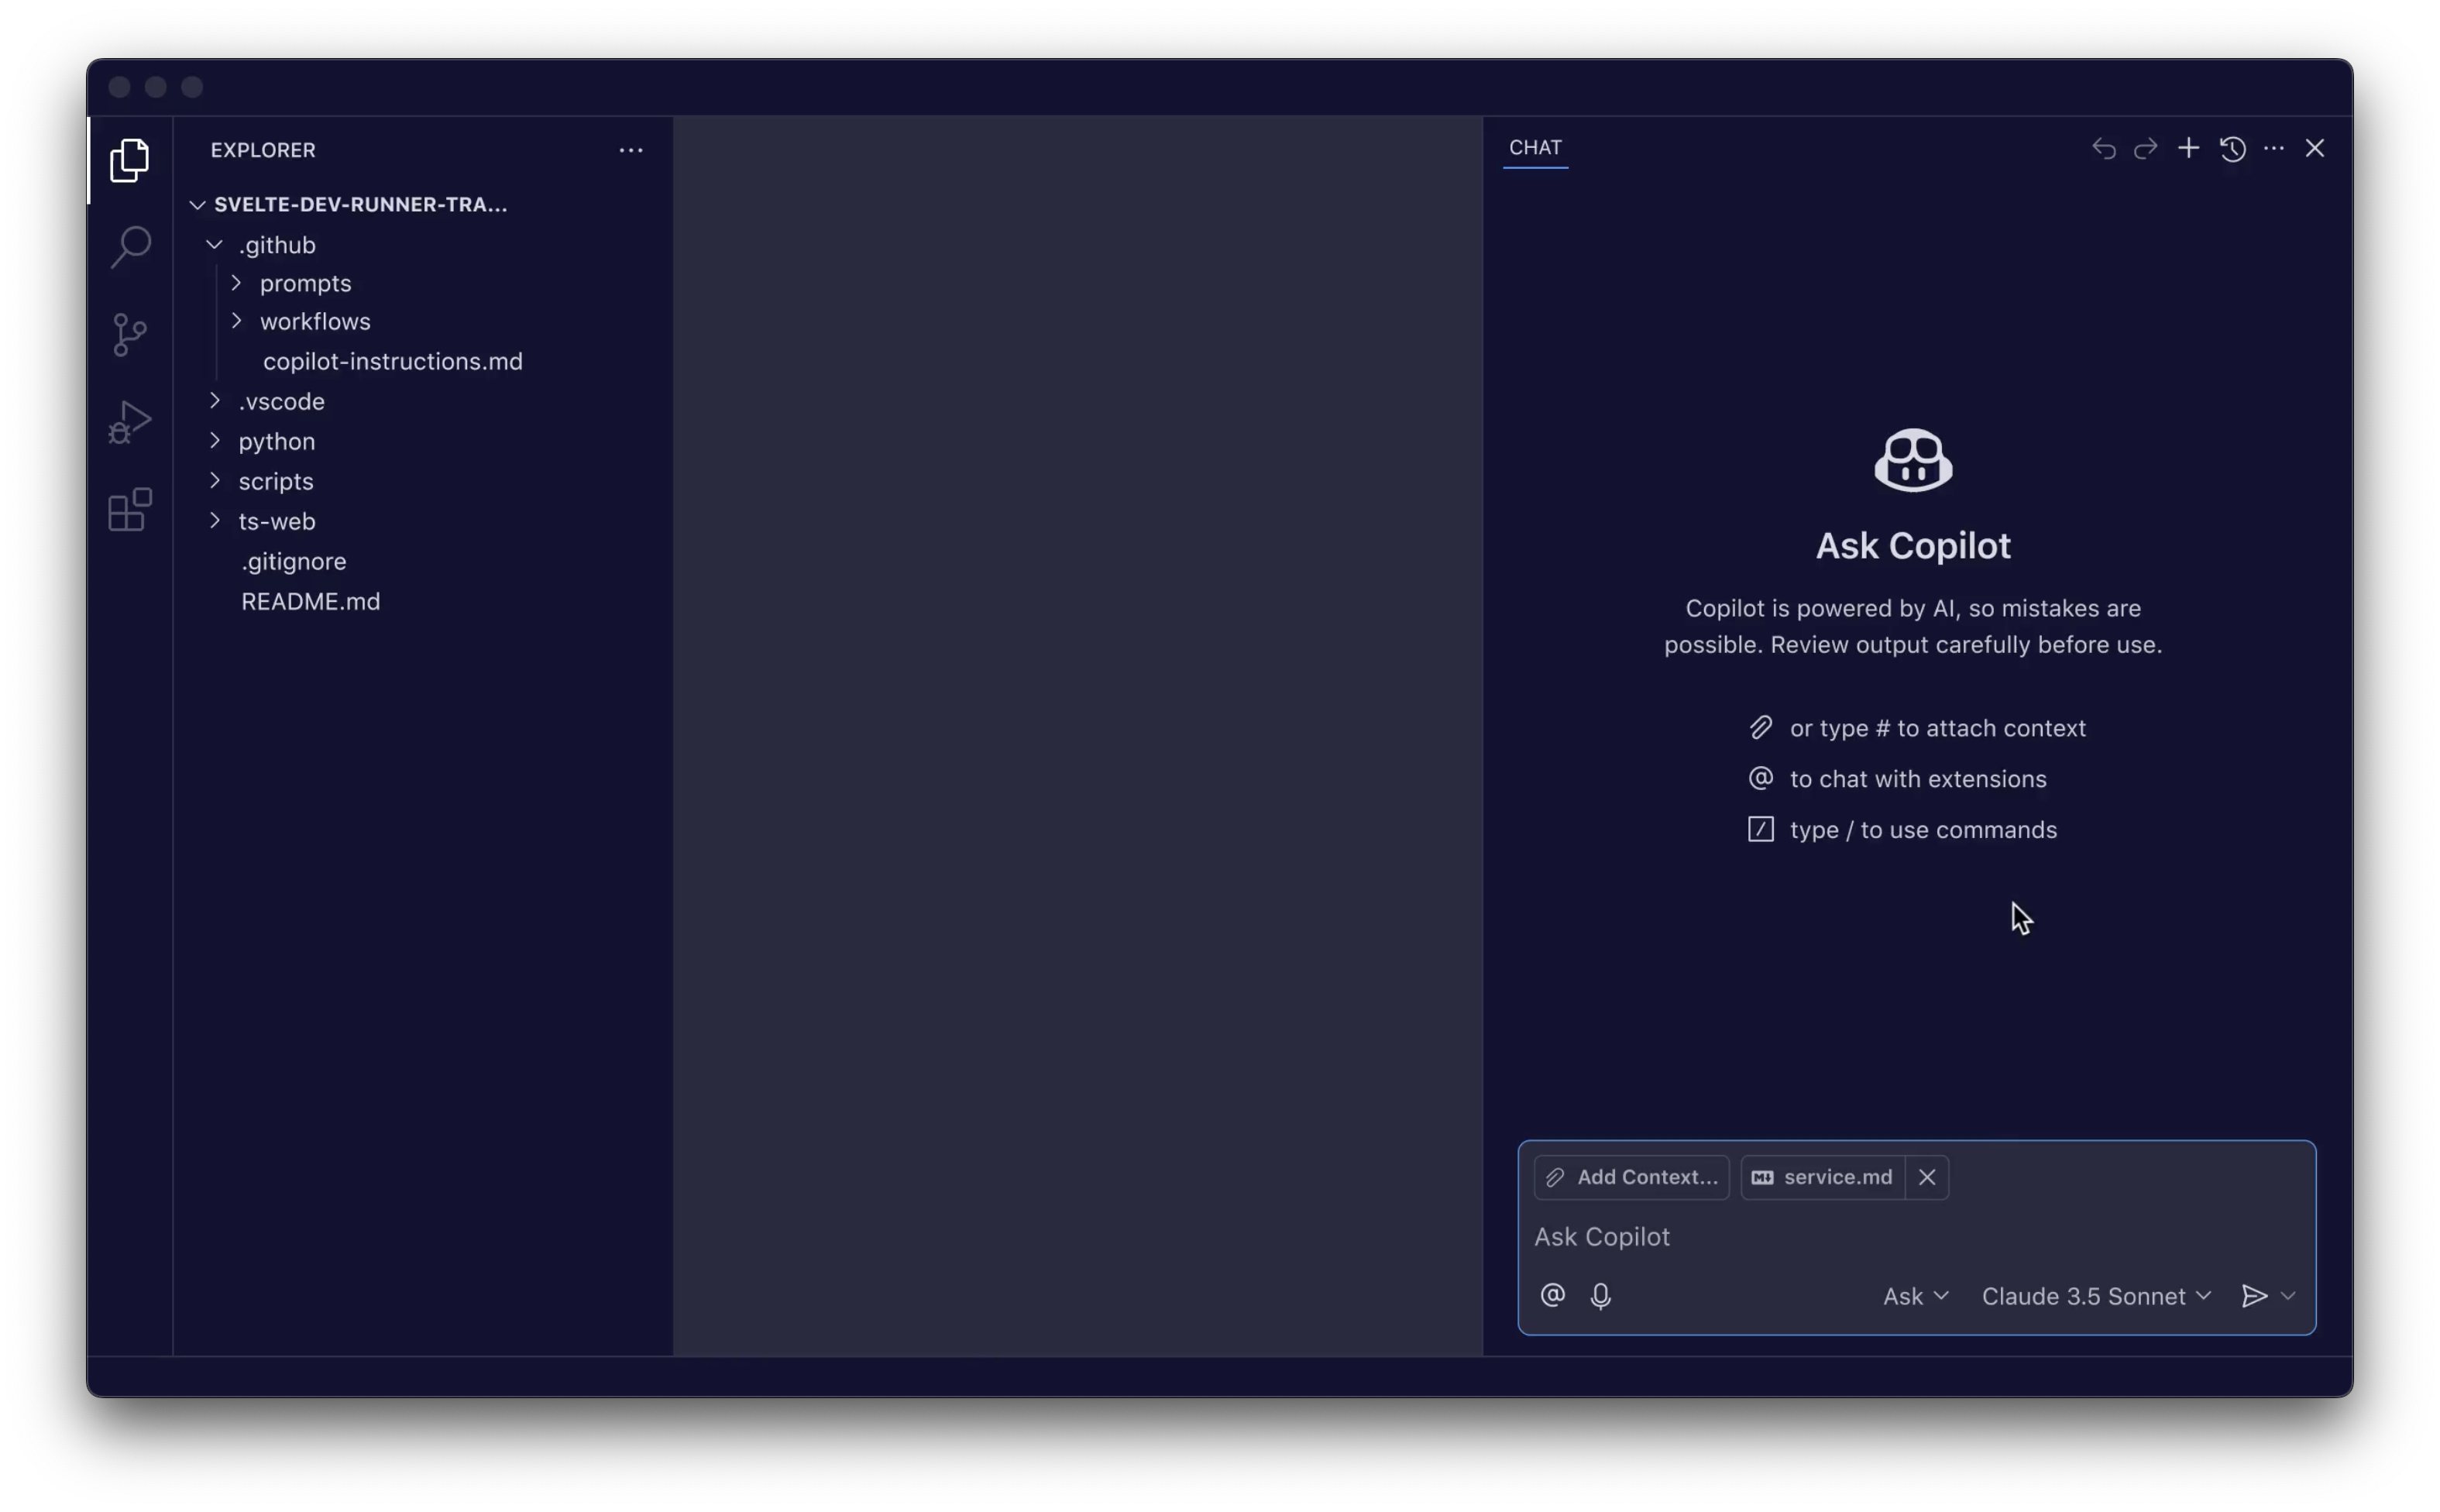
\includegraphics[width=\textwidth]{images/copilot.png}}{VPlayer.swf}

    \end{column}
    \begin{column}{0.45\textwidth}
      \begin{itemize}
        \item Coding agents work largely autonomously
        \item Implement features, fix bugs, write documentation
        \item Powered by large language models (LLMs) fine-tuned for tool use and code generation
        \item Accelerate prototyping
        \item \textbf{Human-in-the-loop is essential}
        \item Can be IDE-integrated, CLI-based, or \textbf{web-based}
      \end{itemize}
    \end{column}
  \end{columns}
\end{frame}

\begin{frame}
  {Coding Agent Examples}
  \begin{columns}
    \begin{column}{0.3\textwidth}
      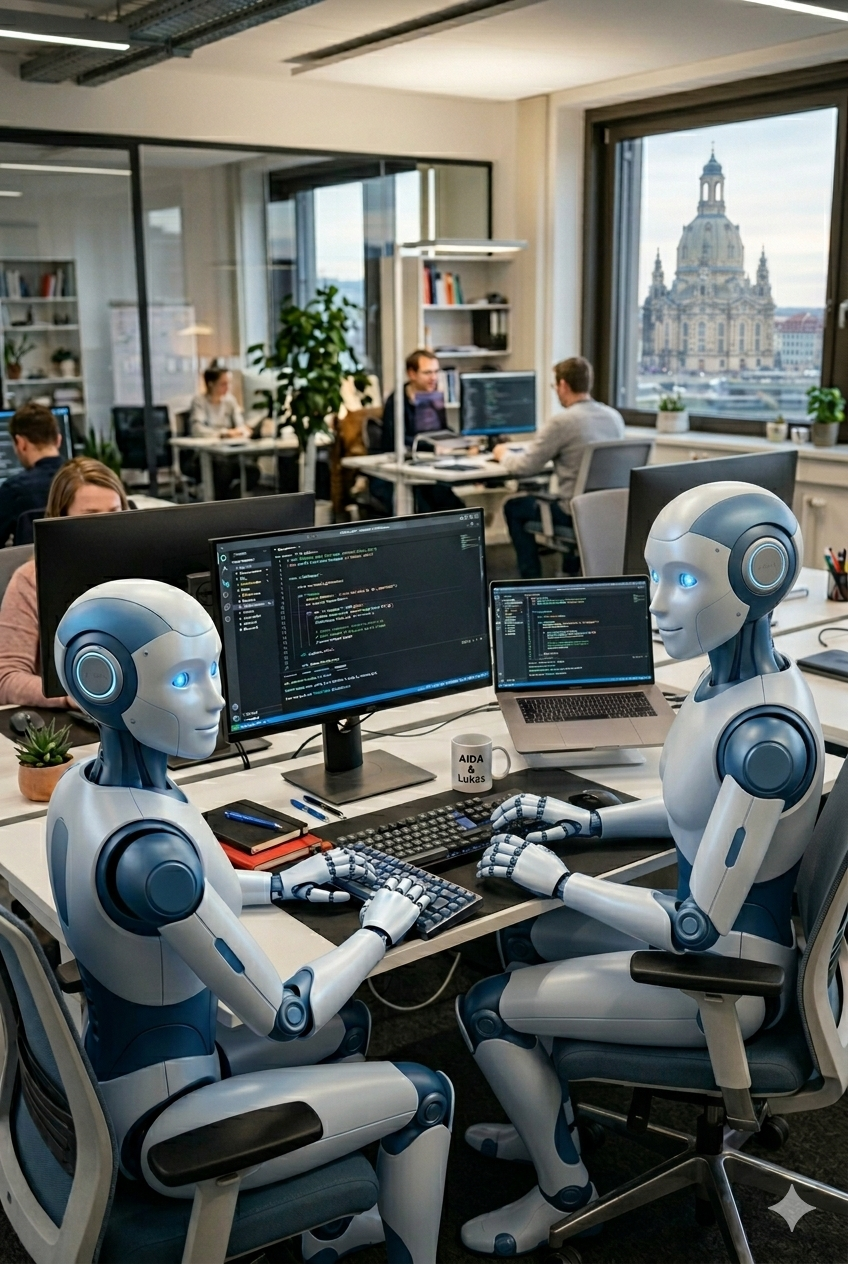
\includegraphics[width=\textwidth]{images/many_agents_at_work_AI_generated.png}
      \tiny AI generated by Gemini Nano Banana 2
    \end{column}
    \begin{column}{0.7\textwidth}
      \Large
      \begin{itemize}
        \item \textbf{GitHub Copilot} (integrated into GitHub, IDE plugin, CLI) \url{https://github.com/features/copilot} easy, good exercise
        \item \textbf{Opencode} (CLI, IDE plugin, GitHub/GitLab CI) \url{https://opencode.ai} \textbf{open source, model-agnostic, self-hostable}
        \item Claude Code (CLI, IDE plugin, App) {\normalsize \url{https://www.anthropic.com/product/claude-code}}
        \item Codex (CLI, IDE plugin, App) \url{https://chatgpt.com/codex}
      \end{itemize}
    \end{column}
  \end{columns}
\end{frame}

\begin{frame}
  {Web-Based Coding Workflow}
  \begin{columns}
    \begin{column}{0.6\textwidth}
      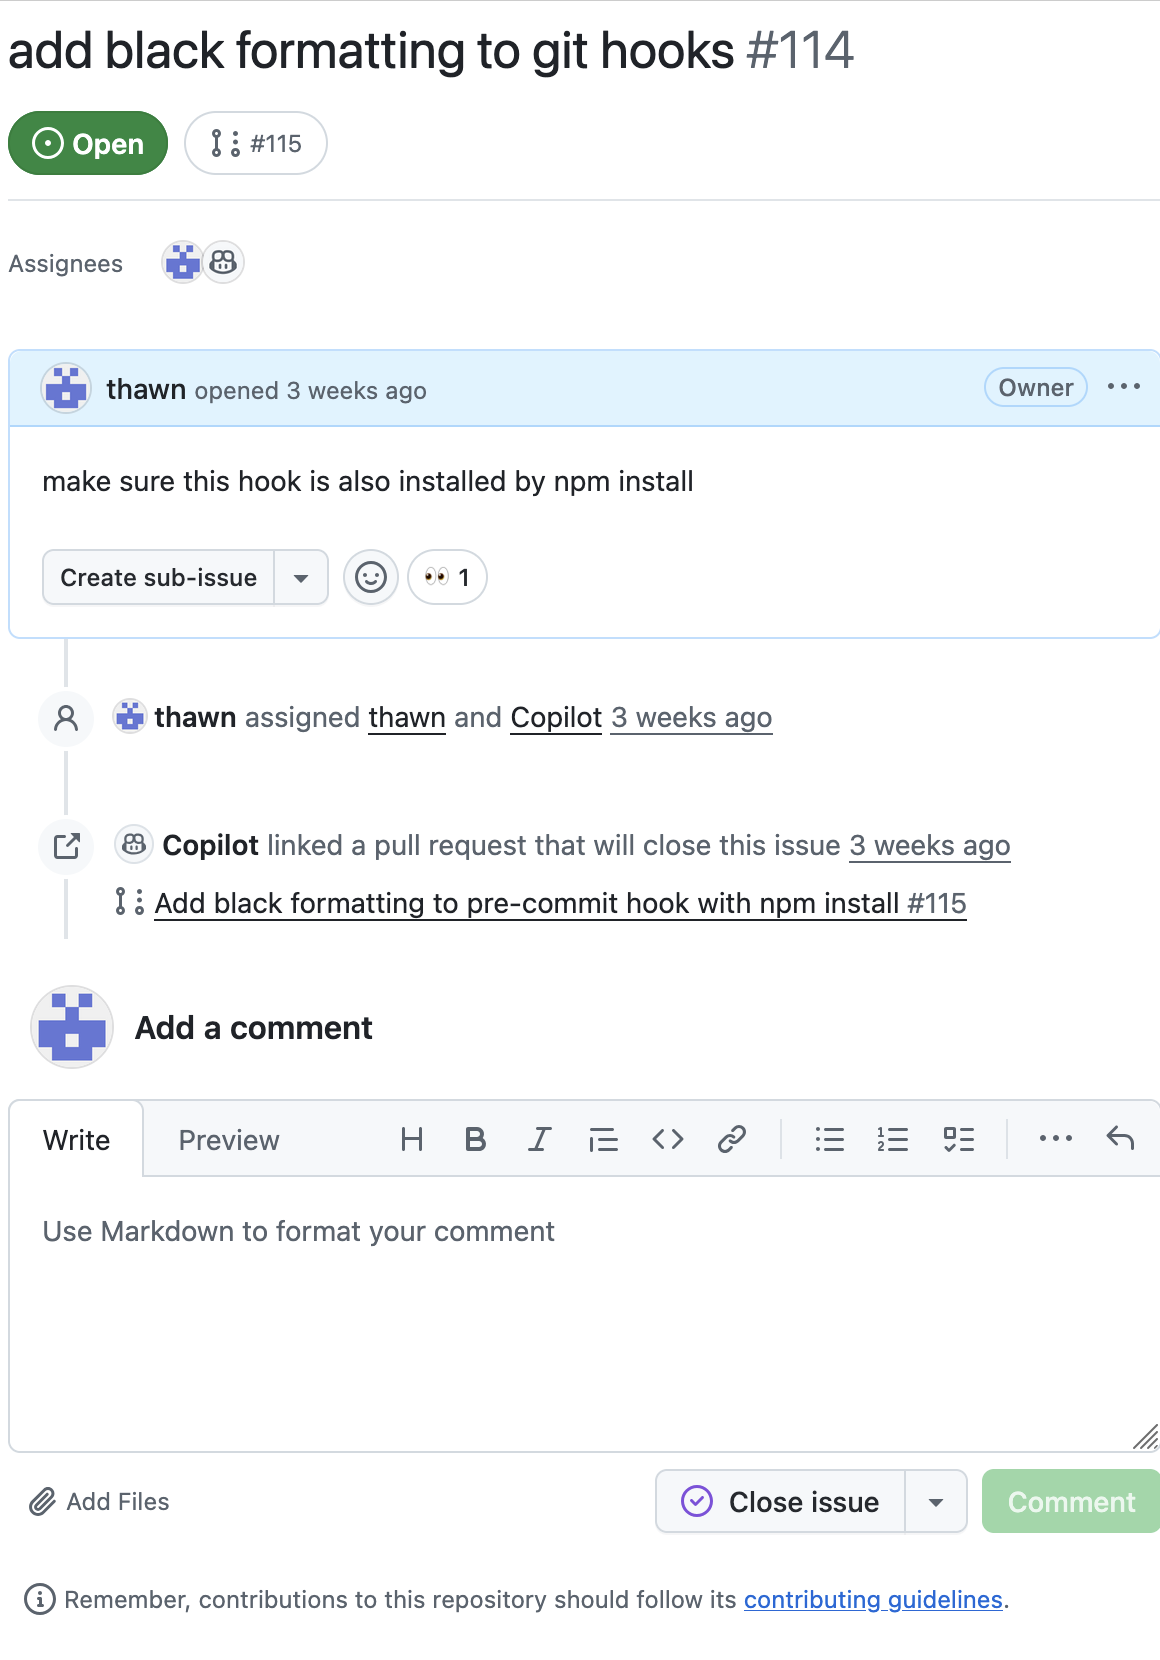
\includegraphics[width=0.49\textwidth]{images/issue.png}
      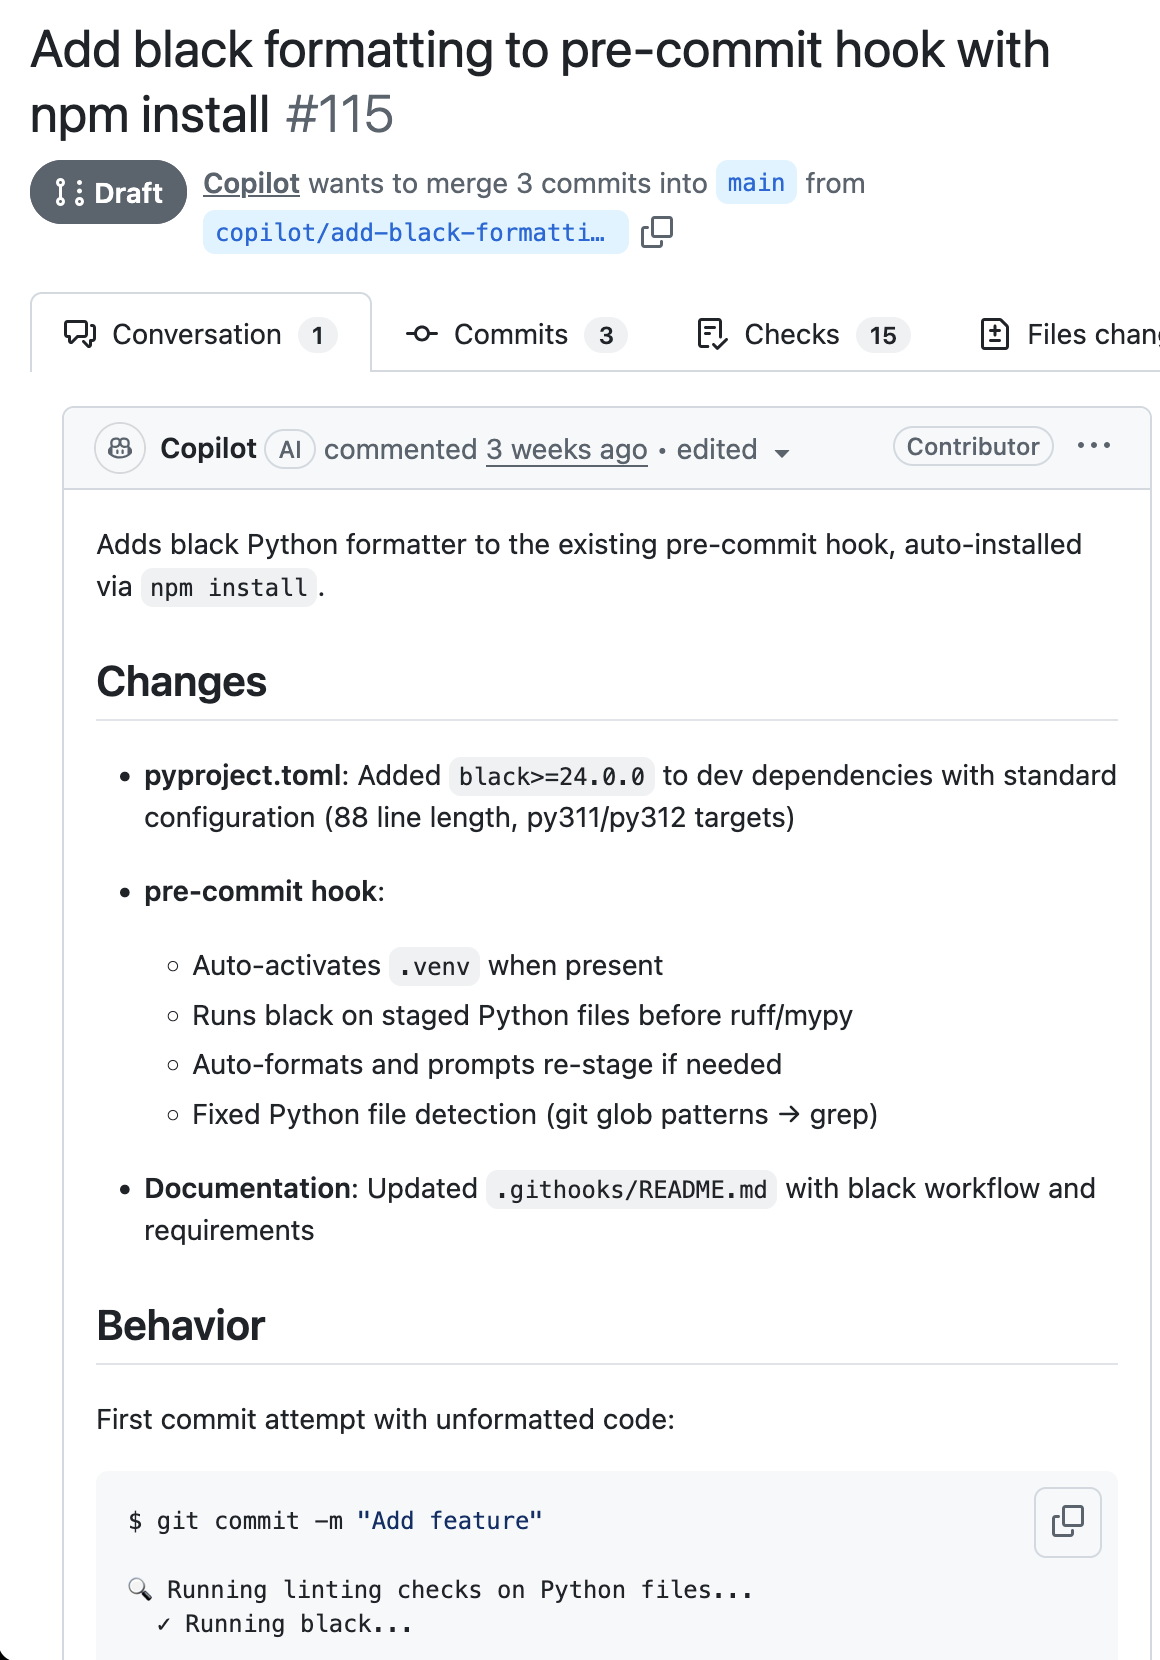
\includegraphics[width=0.49\textwidth]{images/pr.png}
    \end{column}
    \begin{column}{0.4\textwidth}
      \begin{enumerate}[label=\arabic*.]
        \item Open an issue or feature request (e.g., on GitHub).
        \item Assign a coding agent.
        \item The coding agent generates a pull request.
        \item You review, request changes, test, and merge.
        \item This is a great way to practice collaborative coding.
              % \item Let me demonstrate with a live example.
      \end{enumerate}
    \end{column}
  \end{columns}
\end{frame}

% \begin{frame}{Live Demo}

% \end{frame}

\begin{frame}
  {Caveats of Web-Based Coding}
  \begin{columns}
    \begin{column}{0.6\textwidth}
      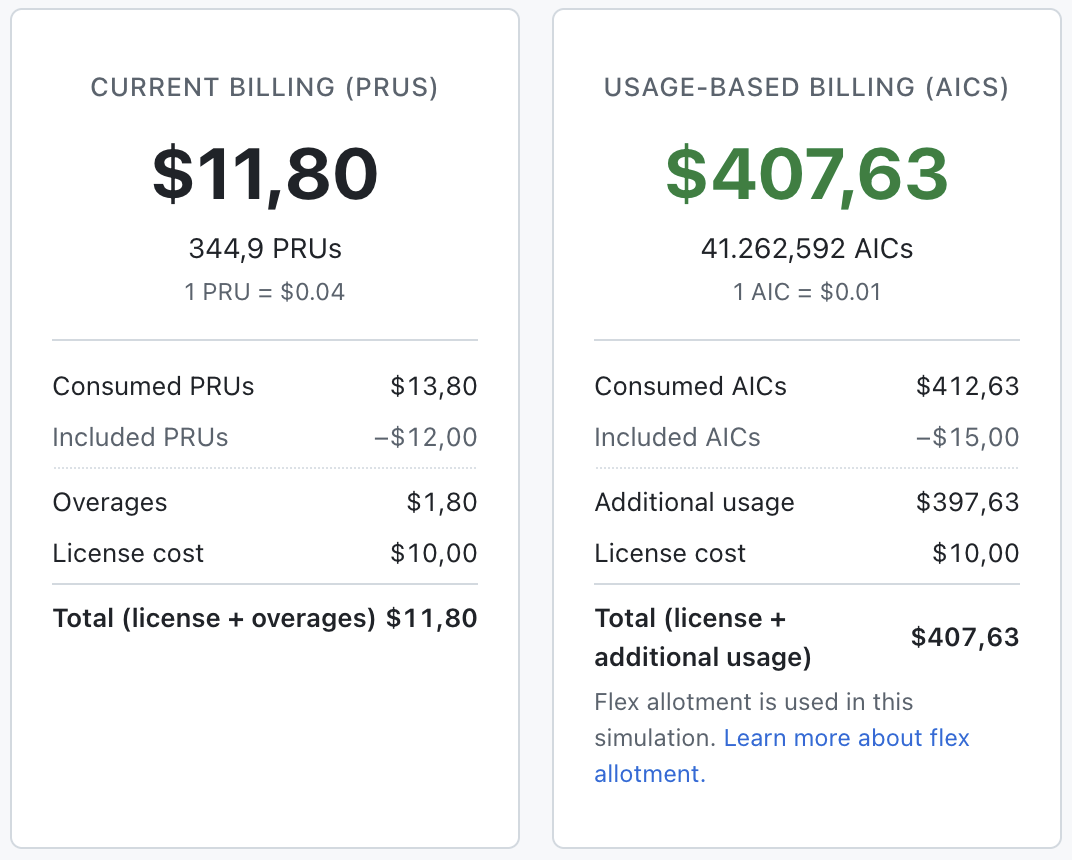
\includegraphics[width=\textwidth]{images/copilot_costs.png}
    \end{column}
    \begin{column}{0.4\textwidth}
      \Large
      \begin{itemize}
        \item Latency: CI runners take $\approx$ a minute to spin up the agent.
        \item Cost: Microsoft just decided to make money instead of subsidizing GitHub Copilot \rightarrow~40 x cost increase. GitLab Duo is a premium feature.
      \end{itemize}
    \end{column}
  \end{columns}
\end{frame}

\begin{frame}
  {Opencode Workflow}
  \begin{columns}
    \begin{column}{0.55\textwidth}
      \includemedia[
        activate=pageopen,
        addresource=images/opencode.mp4,
        flashvars={
            source=images/opencode.mp4
            &autoPlay=true
            &loop=true
          }
      ]{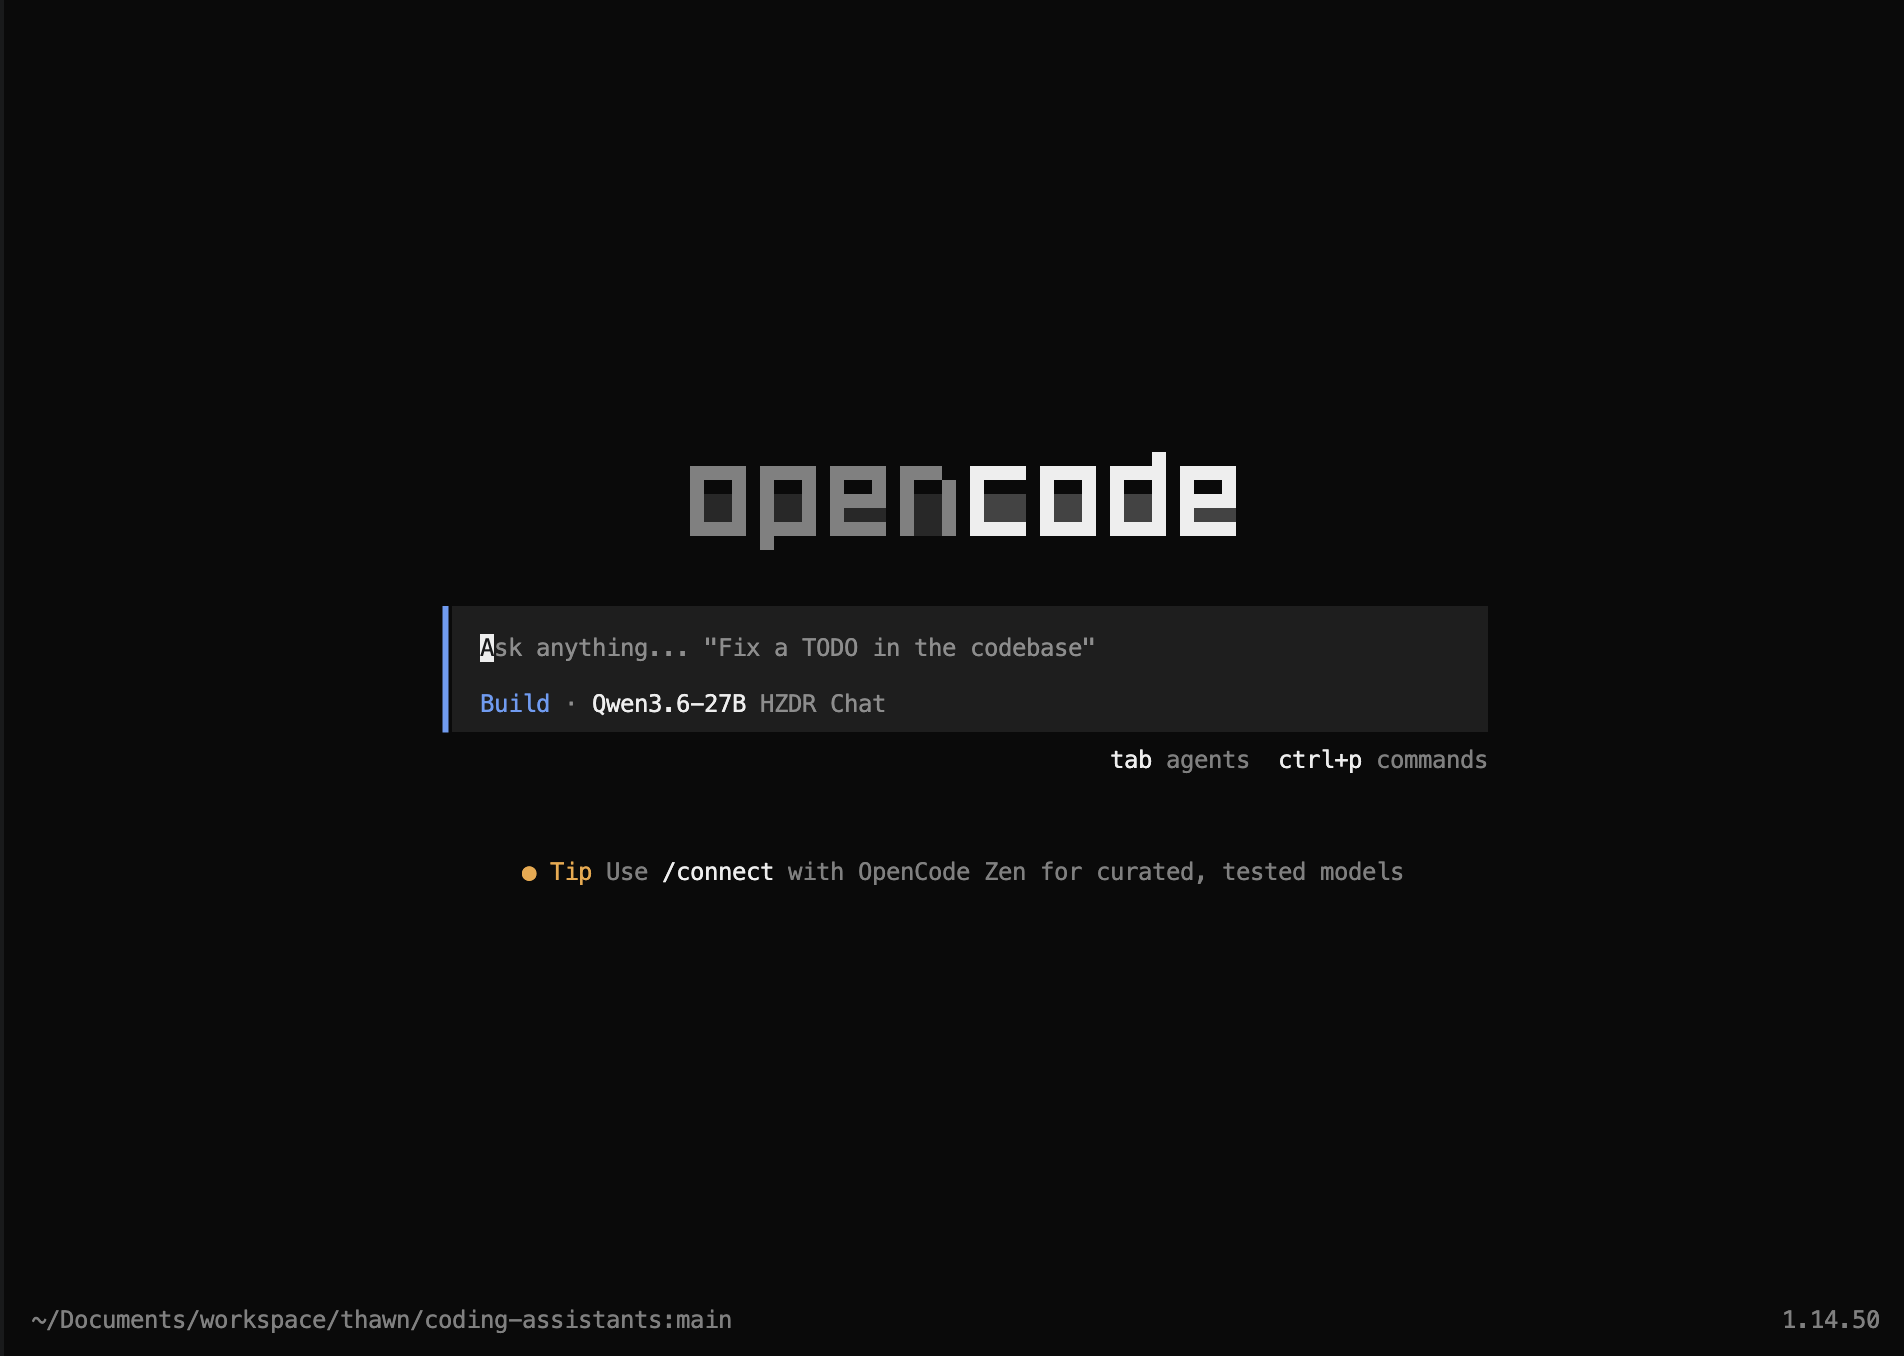
\includegraphics[width=\textwidth]{images/opencode.png}}{VPlayer.swf}

    \end{column}
    \begin{column}{0.45\textwidth}
      \begin{enumerate}[label=\arabic*.]
        \item \textbf{Create a new branch} — \tool{git checkout -b add-new-feature}
        \item \textbf{Plan mode} (\tool{Tab}) — propose changes without executing, iterate with feedback
        \item \textbf{Build mode} (\tool{Tab}) — execute the plan and implement changes
        \item \textbf{Review} — inspect changes, use \tool{/undo} to revert and refine
        \item \textbf{Open a pull request} — opencode can suggest a PR description and title in plan mode
      \end{enumerate}
    \end{column}
  \end{columns}
  \textbf{Never work without version control! (e.g., GitHub, GitLab, or local git)}
\end{frame}

\begin{frame}
  {Best Practices}
  \begin{columns}
    \begin{column}{0.3\textwidth}
      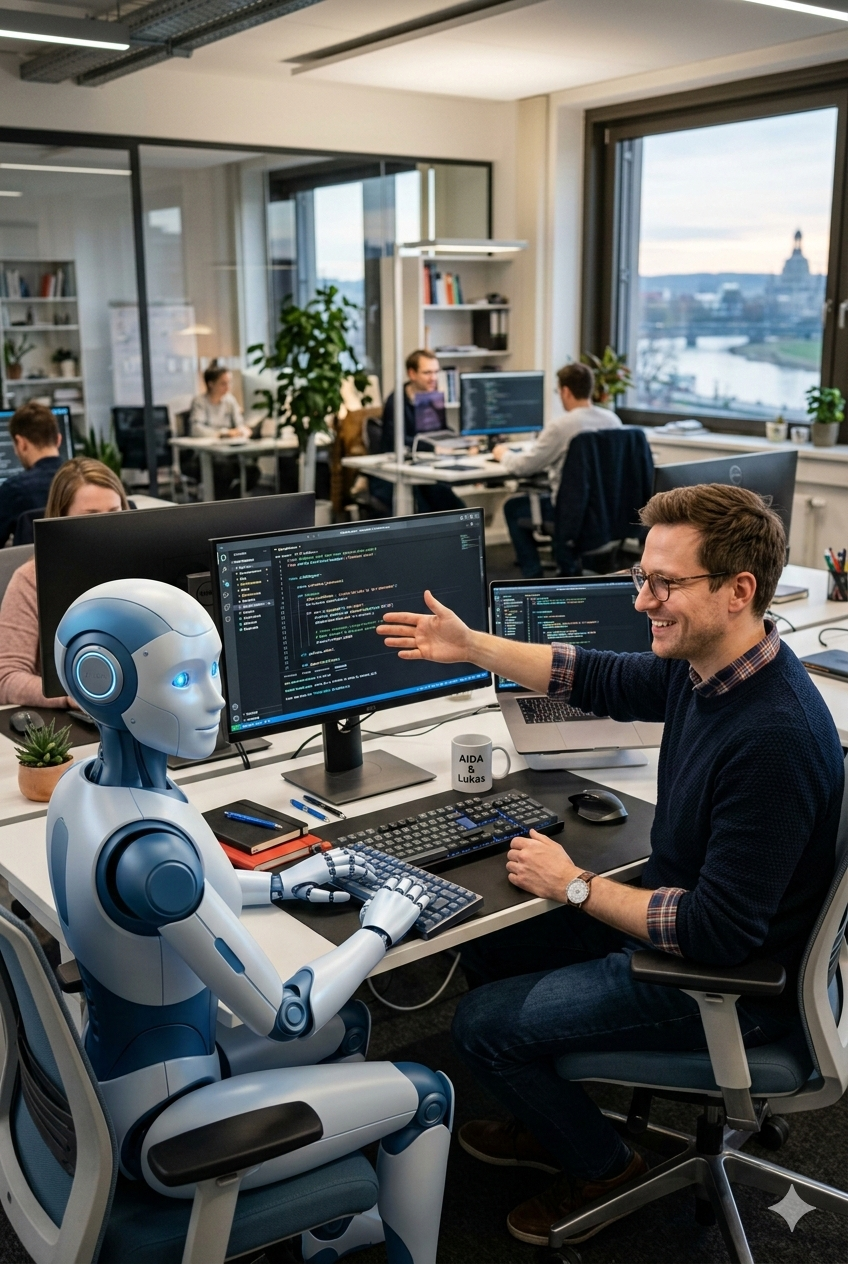
\includegraphics[width=\textwidth]{images/human_instructing_agent_AI_generated.png}
    \end{column}
    \begin{column}{0.7\textwidth}
      \Large
      \begin{itemize}
        \item Specify the desired end result, not how to implement it.
        \item Plan the prompt well (use a chat model).
        \item Use structured tasks and checklists
        \item Understand, review and test all generated code.
        \item Iterate and refine pull requests.
        \item Make sure code is maintainable and secure.
      \end{itemize}
    \end{column}
  \end{columns}
  \tiny AI generated by Gemini Nano Banana 2
\end{frame}

\begin{frame}
  {Writing Maintainable Code}
  \begin{columns}
    \begin{column}{0.6\textwidth}
      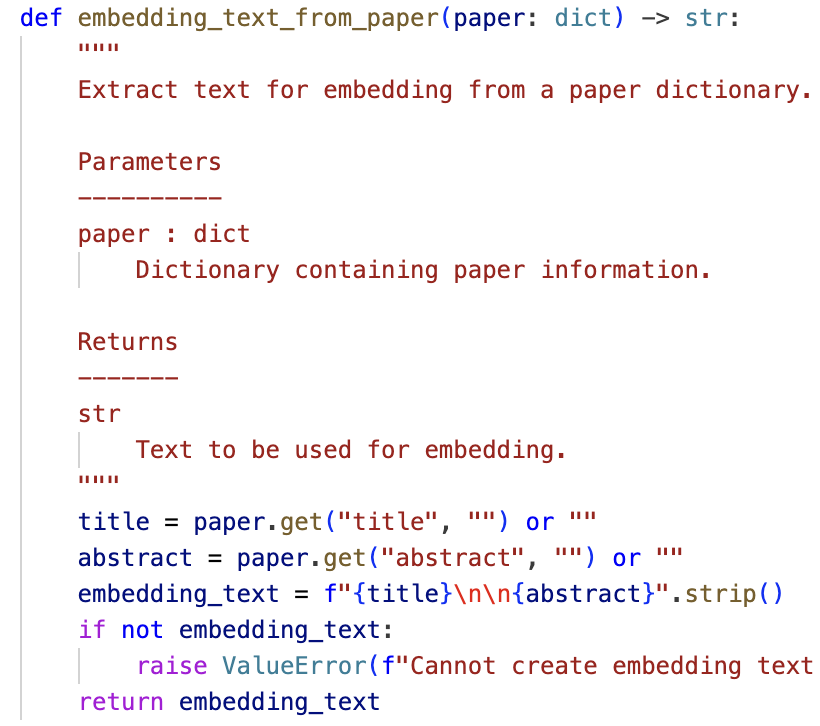
\includegraphics[width=\textwidth]{images/high_quality_code.png}
    \end{column}
    \begin{column}{0.4\textwidth}
      \begin{enumerate}[label=\arabic*.]
        \item \textbf{Documentation}
              \begin{itemize}
                \item Function docstrings
                \item Package documentation
              \end{itemize}
        \item \textbf{Code quality}
              \begin{itemize}
                \item avoid code duplication
                \item modular
                \item testable
                \item type hints
                \item formatters and linters
              \end{itemize}
        \item \textbf{Automated tests}
              \begin{itemize}
                \item unit tests
                \item integration tests
                \item end-to-end tests
              \end{itemize}
      \end{enumerate}
    \end{column}
  \end{columns}
\end{frame}

\begin{frame}
  {Example Prompts to Improve Code Quality}
  \large
  \begin{enumerate}[label=\arabic*.]
    \item Thoroughly examine the code base to improve \textbf{Documentation}
          \begin{itemize}
            \item Add \tool{numpy style} function docstrings
            \item Add \tool{sphinx} documentation including auto-generated API docs
          \end{itemize}
    \item Thoroughly examine the code base to improve \textbf{Code quality}
          \begin{itemize}
            \item add type hints
            \item add git hooks for formatting and linting
            \item remove code duplication
            \item improve code modularity \textrightarrow~aim for $\approx 5$ lines of code per function
            \item improve testability \textrightarrow~avoid global state, and complex dependencies
          \end{itemize}
    \item Add comprehensive \textbf{Automated tests with \tool{pytest}}
          \begin{itemize}
            \item add unit tests \textrightarrow~aim for >90\% coverage
            \item add integration tests
            \item add end-to-end tests for the following workflows: <describe>
          \end{itemize}
  \end{enumerate}
\end{frame}

\begin{frame}
  {Enable Agents to Run Code and Tests}

  \begin{columns}
    \begin{column}{0.3\textwidth}
      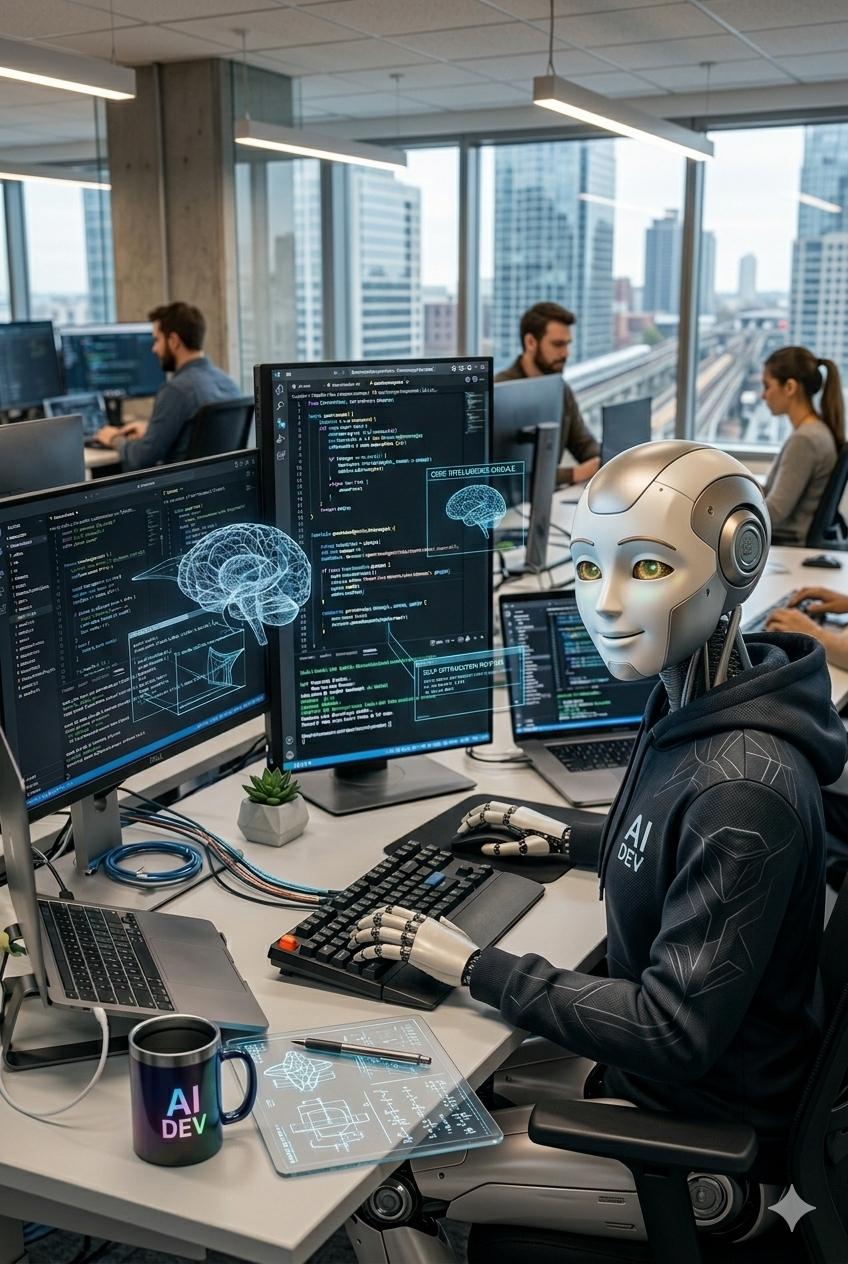
\includegraphics[width=\textwidth]{images/agent_at_work_AI_generated.png}
    \end{column}
    \begin{column}{0.7\textwidth}
      \Large
      \begin{itemize}
        \item Run the agent in an environment where it can execute code and tests
        \item The environment should be safe to execute commands (e.g. a virtual machine or CI runner)
        \item All dependencies to run code and tests should be installed \textrightarrow~on GitHub use \tool{copilot-setup-steps.yml}
        \item Internet access should be restricted to known trustworthy sites to prevent prompt injections
      \end{itemize}
    \end{column}
  \end{columns}
  \tiny AI generated by Gemini Nano Banana 2

\end{frame}

\begin{frame}
  {Coding Agents Improve Productivity}

  \begin{columns}
    \begin{column}{0.3\textwidth}
      
\includegraphics[width=\textwidth]{images/agent_working_with_human_AI_generated.png}
    \end{column}
    \begin{column}{0.7\textwidth}
      \Large
      \begin{itemize}
        \item Initial productivity gain is highest \textrightarrow~80/20 rule becomes 95/5
        \item Ideal for rapid prototyping
        \item Accelerate documentation and testing
        \item Agents have good overview of state-of-the-art \textbf{at the time the model was trained}
        \item Routine coding tasks that are well represented in training data
      \end{itemize}
    \end{column}
  \end{columns}
  \tiny AI generated by Gemini Nano Banana 2

\end{frame}

\begin{frame}
  {Don't Overestimate Coding Agents}

  \begin{columns}
    \begin{column}{0.3\textwidth}
      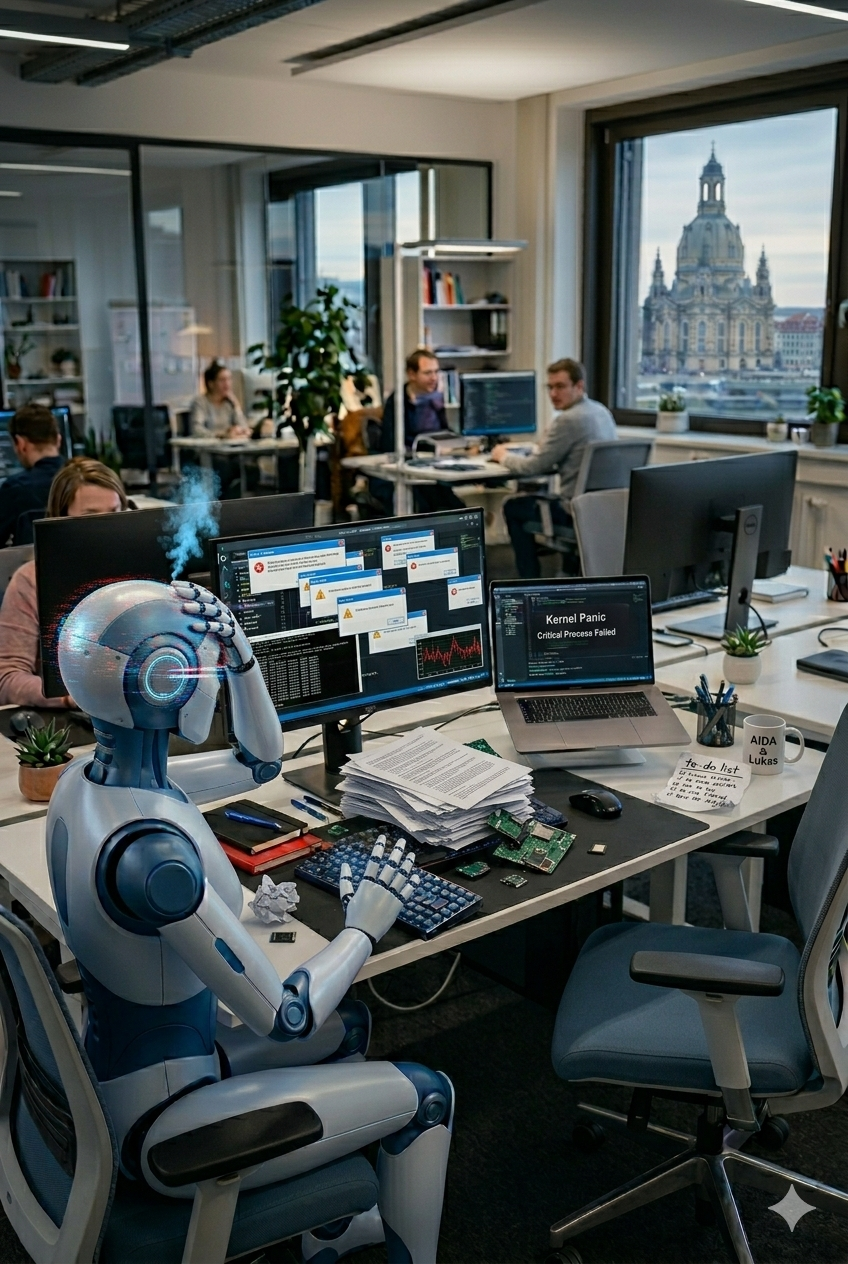
\includegraphics[width=\textwidth]{images/agent_overworked_AI_generated.png}
    \end{column}
    \begin{column}{0.7\textwidth}
      \Large
      \begin{itemize}
        \item Still require human oversight and iteration
        \item Struggle with complex, novel, or poorly specified tasks
        \item Can generate plausible but incorrect code (hallucinations)
        \item Will eventually produce unmaintainable code (duplicate code paths etc.)
        \item Not a replacement for skilled software engineers
      \end{itemize}
    \end{column}
  \end{columns}
  \tiny AI generated by Gemini Nano Banana 2
\end{frame}

\begin{frame}
  {What about coding assistants?}
  \begin{columns}
    \begin{column}{0.6\textwidth}
      \includemedia[
        activate=pageopen,
        addresource=images/use_cases_fast.mp4,
        flashvars={
            source=images/use_cases_fast.mp4
            &autoPlay=true
            &loop=true
          }
      ]{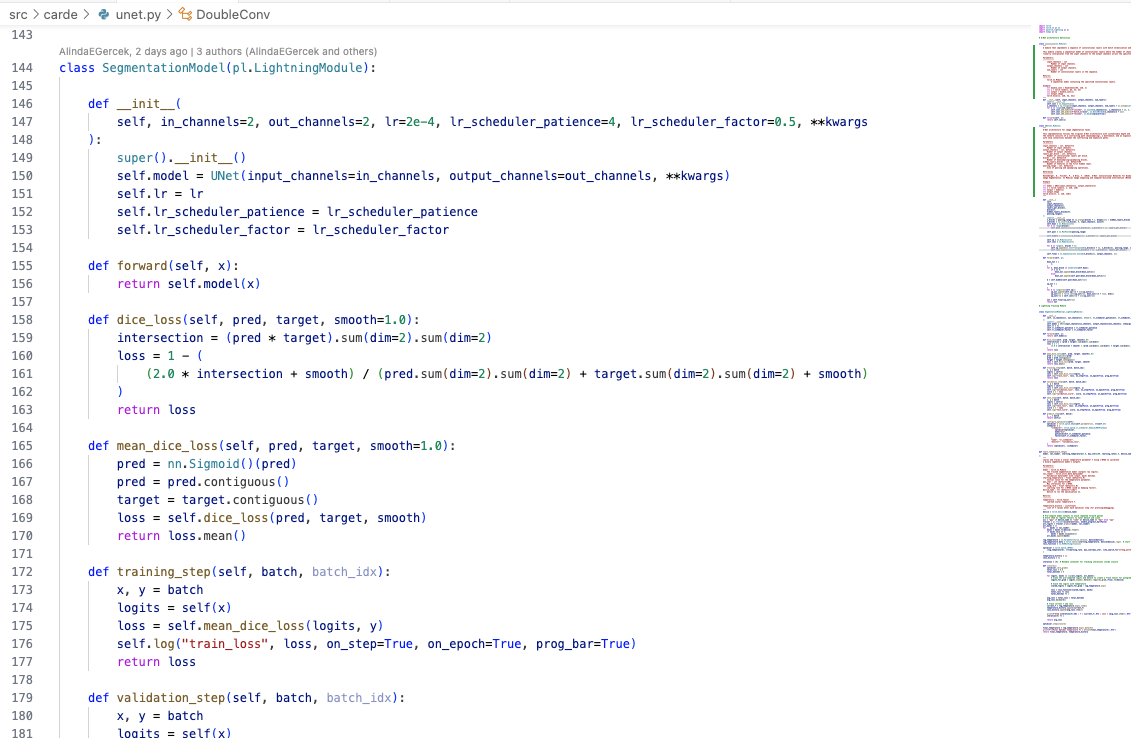
\includegraphics[width=\textwidth]{images/add_nll_loss.png}}{VPlayer.swf}
    \end{column}
    \begin{column}{0.4\textwidth}
      \begin{itemize}
        \item IDE-integrated tools that suggest code, document, refactor, explain, and generate tests.
        \item Powered by smaller large language models (LLMs) trained for code generation.
        \item Still useful to accelerate daily coding
      \end{itemize}
    \end{column}
  \end{columns}
\end{frame}

\begin{frame}
  {Summary}

  \begin{columns}
    \begin{column}{0.3\textwidth}
      
\includegraphics[width=\textwidth]{images/QR-code_github_repo.png}
      \url{https://github.com/thawn/coding-assistants} CC-BY 4.0
    \end{column}
    \begin{column}{0.7\textwidth}
      \Large
      \begin{itemize}
        \item Coding agents accelerate software development
        \item Require careful prompting and human oversight
        \item Ideal for rapid prototyping, documentation, and testing
        \item Struggle with complex or novel tasks
        \item No replacement for skilled software engineers
      \end{itemize}
    \end{column}
  \end{columns}
\end{frame}

\begin{frame}
  {Hands-on Exercise: Build Your Own Software}
  \begin{itemize}
    \Large
    \item Use Opencode or GitHub Copilot for a small project. Examples:
          \begin{itemize}
            \item Implement the research proposal or visualization example from session two
            \item Write a script to automate a tedious task in your daily work
            \item Implement a new feature in an existing codebase
            \item Fix a bug
            \item Write documentation for a project
            \item Implement unit tests for an existing codebase
            \item Revive a legacy project by migrating it to a modern language or framework
          \end{itemize}
  \end{itemize}
\end{frame}

\end{document}
